\documentclass[conference]{IEEEtran}
\usepackage{longtable}
\usepackage{graphicx}
\usepackage{graphics}
\usepackage{float}
\usepackage{cite}
\usepackage{amsmath,amssymb,amsfonts}
\usepackage{algorithmic}
\usepackage{graphicx}
\usepackage{textcomp}
\usepackage{xcolor}
\usepackage{dblfloatfix}
\usepackage{cleveref}
% \usepackage{algpseudocode}
\usepackage{xcolor}
\usepackage[linesnumbered,ruled,vlined]{algorithm2e}

\title{Halfway Evaluation Master thesis: Design an algorithm to optimize the metro ring network for real-life applications based on user demands}
\author{\IEEEauthorblockN{Luong Quoc Dat}
\IEEEauthorblockA{\textit{Dept. of Electrical Engineering} \\
\textit{Technical University of Eindhoven}\\
}}
\date{Feb 2021}

\makeatletter
\newcommand{\removelatexerror}{\let\@latex@error\@gobble}
\makeatother

%%% Coloring the comment as blue
\newcommand\mycommfont[1]{\footnotesize\ttfamily\textcolor{blue}{#1}}
\SetCommentSty{mycommfont}

\SetKwInput{KwInput}{Input}                % Set the Input
\SetKwInput{KwOutput}{Output}              % set the Output


\begin{document}
\maketitle

\begin{abstract}
This document is a halfway evaluation of the master thesis: Design an algorithm to optimize the metro ring network for real-life applications based on user demands. In this work, the real applications deployment, user traffic pattern generation software, traffic captured from each application as well as aggregated traffic and simulation software design are presented.   
\end{abstract}

% \begin{IEEEkeywords}
% component, formatting, style, styling, insert
% \end{IEEEkeywords}

\section{Introduction}
\label{sec:Introduction}
% section Introduction (begin)
In recent years, it is undeniable that there is a significant increasing trend in the number of users as well as devices connected to the Internet \cite{International2017}. This trend leads to huge demands in optical metro networks infrastructure in terms of service expectations. Therefore, optical metro networks should efficiently support a variety of access applications with different dynamic user traffic patterns from various sources such as enterprises, home applications, media streaming, and IoT applications. These applications not only require high bandwidth demands but also they require low latency response. To address this issue, one solution that could think of is edge computing. 

Edge computing refers to the enabling technologies that allow computation to be performed at the metro network so that computing happens near data sources. It works on both downstream data on behalf of cloud services and upstream data on behalf of IoT services. Edge computing can be any computing or networking resource residing between data sources and cloud-based data centers. For example, in a metro network, an optical metro node can be equipped with a powerful server as an edge computing and handle requests and responses between users and the cloud datacenters. In edge computing, the end device not only consumes data but also produces data. And at the network edge, devices not only request services and information from the cloud but also handle computing tasks including processing, storage, caching. Edge computing could yield many benefits. The most important benefit is reducing application latency. For instance, researchers built a proof-of-concept platform to run a face recognition application in \cite{7372286}, and the response time is reduced from 900 to 169 ms by moving computation from cloud to the edge. Researchers in \cite{5280678} also have shown that using edge computing to offload computing tasks for wearable cognitive-assistance systems improves response times by between 80 and 200 ms and reduces energy consumption by 30 to 40 percent.

In the TU/e lab, there is an experiment has been carried based on SDN reconfigurable and network slicing to enable optical metro access ring network with edge computing resources \cite{8818041}. In this experimental set up, in Figure \ref{fig:metro_ring}, B. Pan \textit{et. al.} has been demonstrated that using SDN, the MCU-based OpenROADM agents can be controlled via NETCONF protocol, which in turn, gives the command to FPGA via PCIE data flow. The FPGA will drive SOAs to control the traffic inside the optical switch. The classification algorithm based on the utilization of network resources, if it is a slightly loaded application can be hosted in an edge computing node, if it is fully loaded the insensitive application is switched to centralized DC to save resources for the latency-sensitive application.

However, in the demonstration, there were only 2 applications and there was no real-life user pattern considered. Meanwhile in the future, with real traffic from various applications and rather complicated network status, such as link utilization, latency, and packet loss, we need an algorithm that can allocate the applications in different nodes in a more efficient way to serve users' requests. To solve this problem, this project aims to develop an algorithm, which is based on different application requirements and user demands, to optimize the deployment of applications in the optical metro network to satisfy service expectations.


\begin{figure*}[hbtp]
\centering
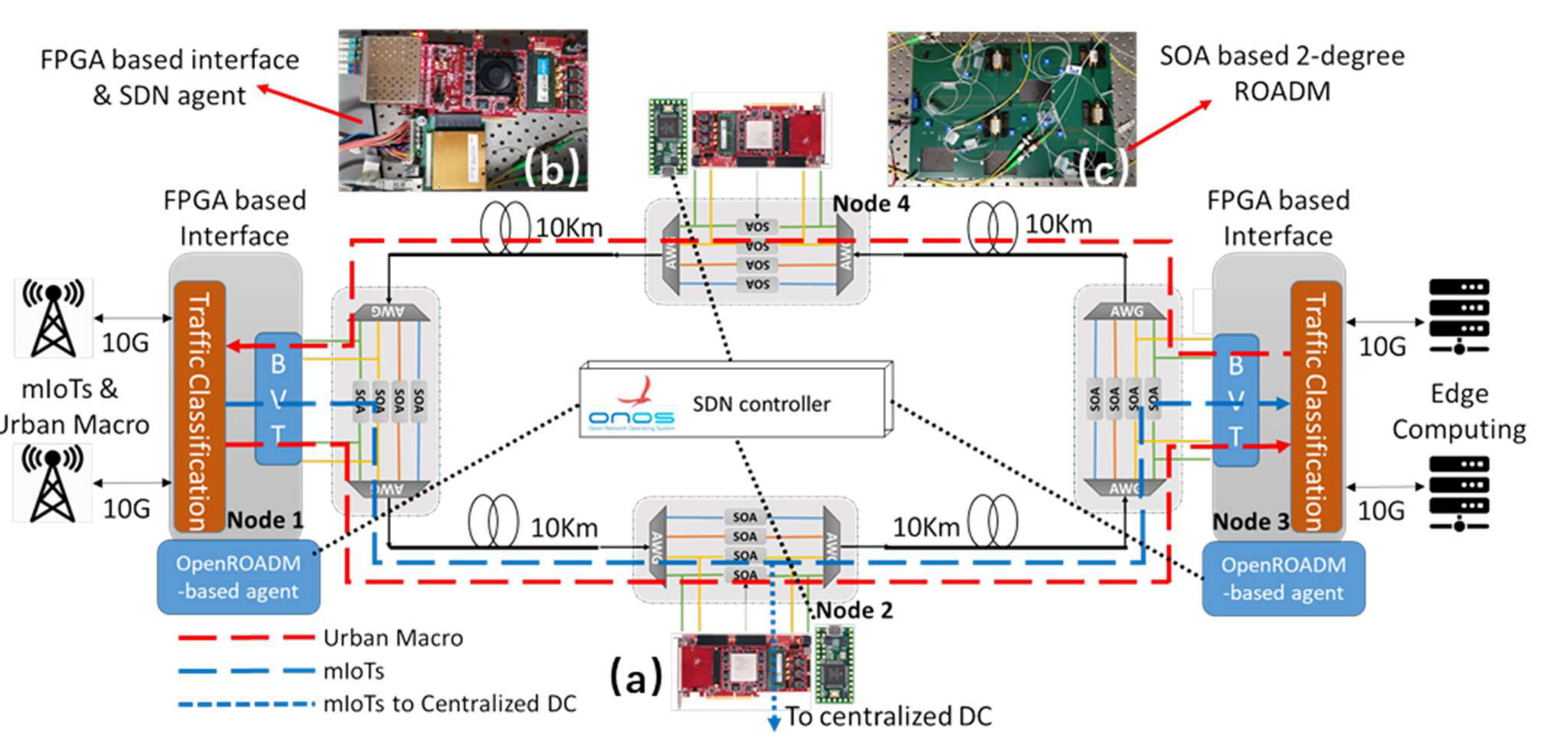
\includegraphics[scale = 0.4]{imgs/ring_metro_network.png}
\caption{Metro Ring Network}
\label{fig:metro_ring}
\end{figure*}

% section Introduction (end)

\section{Thesis Objective}
\label{sec:Thesis Objective}
% section Thesis Objective (begin)
The project's main objective is to develop a software algorithm to control where should the applications deployed in the network to satisfy the application requirements. The software will be developed, simulated, and tested. To achieve the thesis objective, the project has the following main tasks:
\begin{itemize}
    \item Deploy real-life applications in the optical network.
    \item Develop user traffic generation software for each application.
    \item Set up an experiment to collect traffic data in the metro ring network.
    \item Develop network simulation software based on data collected in the experiment.
    \item Develop algorithm and test with simulation.
    \item Train the algorithm online with the real data from the experiment.
\end{itemize}

% section Thesis Objective (end)

% \section{Literature review}
% \label{sec:Literature review}
% % section Literature review (begin)

% Just find a lot of papers and they used DRL algorithmn to fix allocate the VNF

% Docker container technology.

% 1. About the resource allocation using the different algorithm? 
% heuristic ? 
% meta heuristic?
% DRL?
% compare the difference and advantages and disadvantages!

% 2. Inside the DRL? what is the most used? why should we use that algorithm?
% compare inside the DRL algorithms?

% % section Literature review (end)

\section{Experiment set up}
\label{sec:Experiment set up}
% section Experiment set up (begin)
\subsection{Ring Metro Network set up}

As we can see from the Figure \ref{fig:metro_ring} and Figure \ref{fig:full_metro_ring}, the ring optical metro network consists of 4 nodes connect to each other by a 10Gbps unidirectional optical link (red lines). Each node consists of the optical part which is SOA-based 2-degree ROADM, FPGA controller with O/E/O interfaces, and a powerful server for computing.  The traffic that comes from the access network will be aggregated to the metro network. There is also an optical link to the data center that has been set up in the lab.

\begin{figure}[]
    \centering
        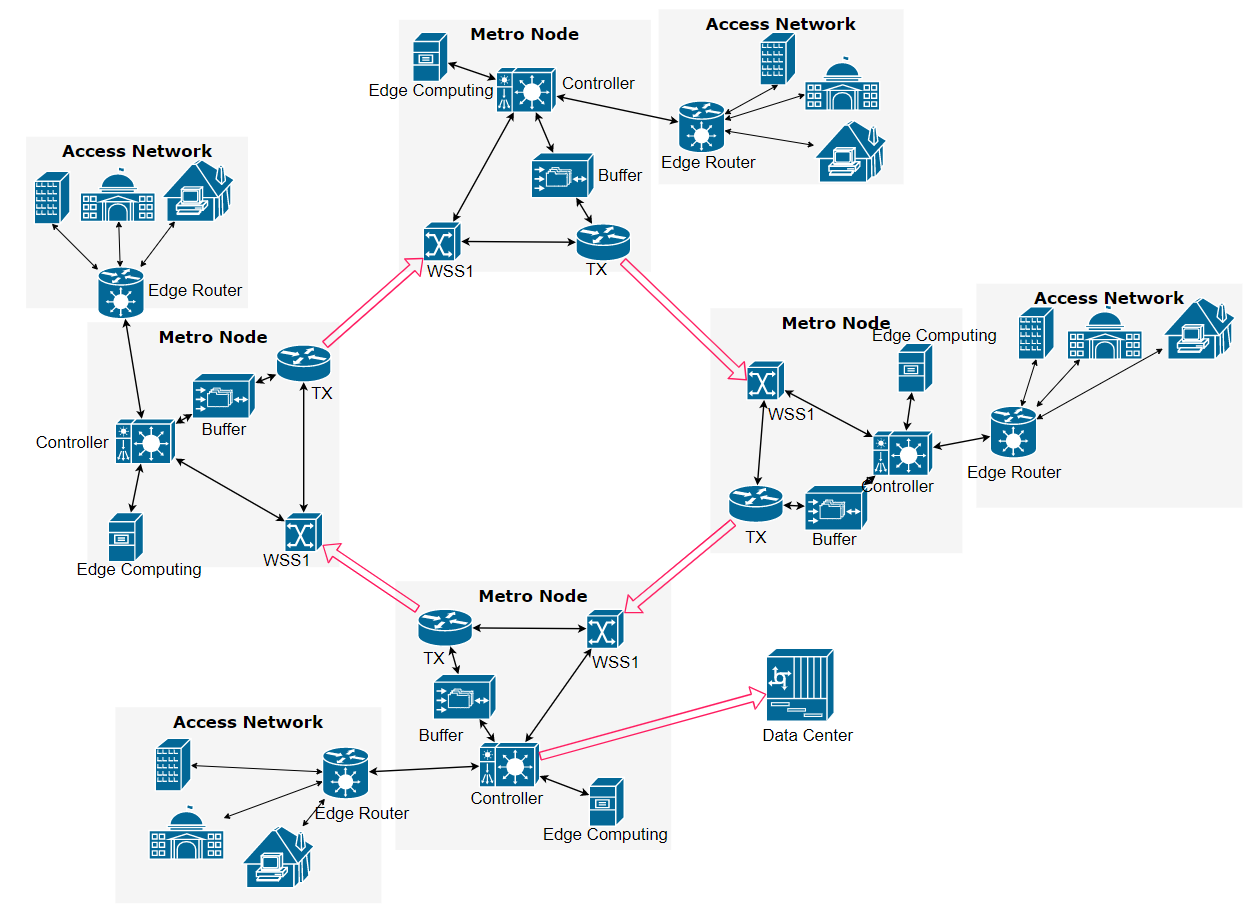
\includegraphics[scale = 0.25]{imgs/metro_ring_with_DC.png}
        \caption{Metro Ring Network}
        \label{fig:full_metro_ring}
    \end{figure}

\subsection{Applications}

There are many usage cases of edge computing in real-life represented in various papers \cite{International2017, 7469991, Shi2016}. Among the applications that could be deployed in the optical metro network, web searching, web serving, and online shopping are chosen. They used the most popular platform on the Internet today: Nginx server, which has taken from Apache since April 2019 \cite{netcraft_news_2021}. To deploy all these real application servers to the optical metro network, we have 2 options: container and virtual machine. In this work, all the applications are deployed using docker container technology. 

A container is a standard unit of software that packages up code and all its dependencies so the application runs quickly and reliably from one computing environment to another. A Docker container image is a lightweight, standalone, executable package of software that includes everything needed to run an application: code, runtime, system tools, system libraries, and settings. Containers and virtual machines have similar resource isolation and allocation benefits but function differently because containers virtualize the operating system instead of hardware. Containers are more portable and efficient \cite{7036275}.

Containers are an abstraction at the app layer that packages code and dependencies together. Multiple containers can run on the same machine and share the OS kernel with other containers, each running as isolated processes in userspace. As in Figure \ref{fig:container_img}, containers take up less space than VMs (container images are typically tens of MBs in size), can handle more applications, and require fewer VMs and Operating systems \cite{docker}.

\begin{figure}[]
    \centering
        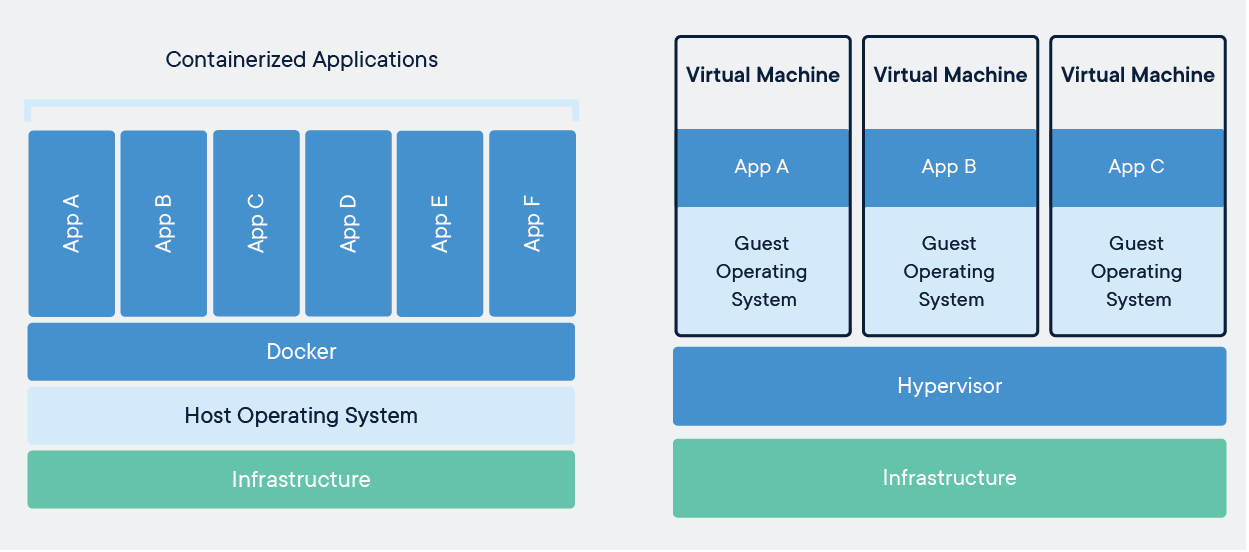
\includegraphics[scale = 0.25]{imgs/container-VM.png}
        \caption{Container and Virtual Machine}
        \label{fig:container_img}
    \end{figure}

The application servers can be deployed in any node in the network. Because the access network is not available in the lab, simulated traffic is generated from the server in each node to the metro network as user simulator containers. Both application servers and users for each application server are containerized in docker containers as in Figure \ref{fig:real_set_up}.

\begin{figure}[]
\centering
    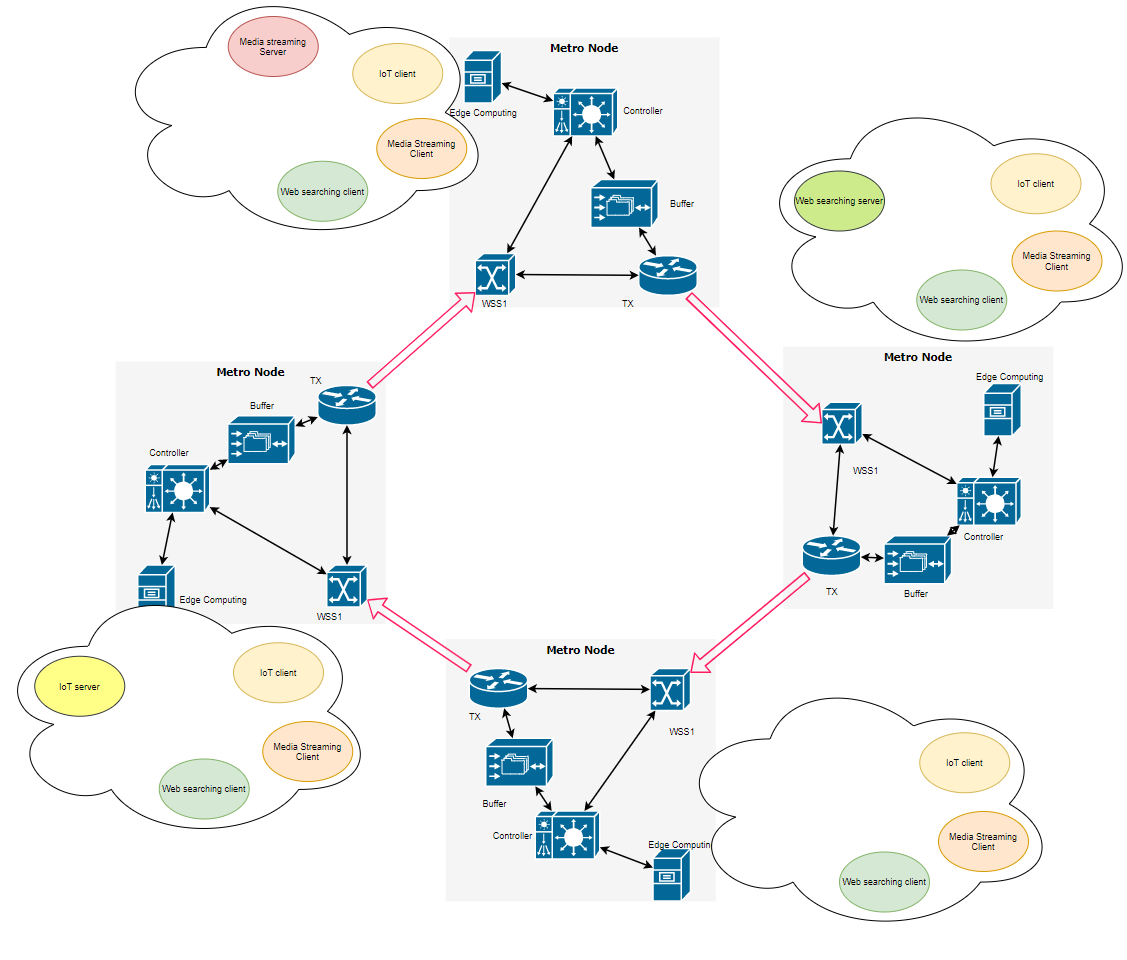
\includegraphics[scale = 0.25]{imgs/real_experiment_set_up.png}
    \caption{Metro Ring Network}
    \label{fig:real_set_up}
\end{figure}

To build an effective algorithm that determines which node each application server should be, the bandwidth that each application server occupies based on real user requests is captured. To capture the traffic between each application and its user, node 3 and node 4 have been used to experiment as we can see in Figure \ref{fig:server_deployment}. In the experiment, we captured each application at a time.

In the media streaming server, an HD video 1080p resolution length of 5.15 minutes is stored in the Nginx server and ready to be requested from the user simulator. Similarly, for web serving, web searching, and online shopping, there is a website page of Wikipedia, google result page and amazon frontpage HTML file is stored inside the Nginx server, respectively.

\begin{figure}[]
    \centering
        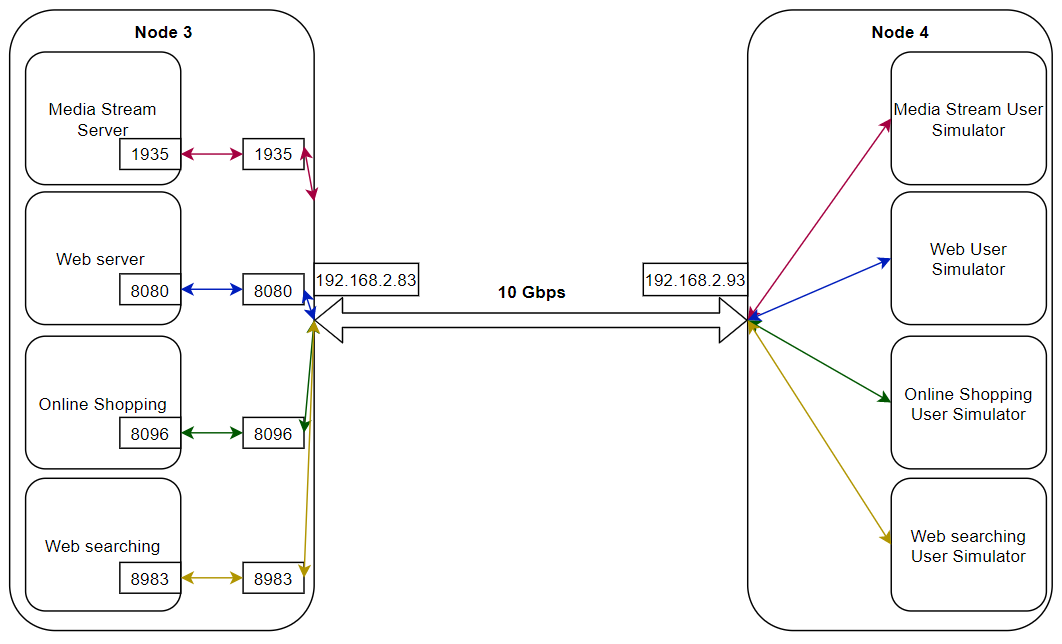
\includegraphics[scale = 0.3]{imgs/server_deployment.png}
        \caption{Application and client Containers in node 3 and 4}
        \label{fig:server_deployment}
    \end{figure}

\subsection{User traffic generator}
To the most knowledge of the author, most of the user behavior can be assumed daily periodic based on research papers \cite{Kooti2016,Ullah2012,Taghavi2012,Yu2006}. Based on the patterns in these researches, a software program python-based has been constructed to simulate the user. To simulate multiple concurrent users at the same time we used multi-threading in python. Each thread represents a user. The algorithm to generate users for each application is represented in Algorithm \ref{algo:user-traffic-gen}. 

For each different server application, we used different tools to make user requests. For media streaming (Nginx server), RTMP protocol and FFmpeg has been used to send request from each user thread. For web searching, web serving, and online shopping, the user requests are HTTP protocol and python packages for HTTP requests have been used. Noted that FFmpeg needed to be configured to remove codec processing from the default setting to reduce the CPU consumption on the host server.

\removelatexerror
\begin{algorithm}[]
    \DontPrintSemicolon
        \KwInput{Number of concurrent active users hourly in 1 day}
        \KwOutput{User threads hourly}
        
        User thread:
        \While {True}
        {
            Send a request to the server.

            Sleep(Read/watch duration)
        }

        Initial: Create an initial number of user threads based on 1st day.

        \For{each day in our simulation time}
        {
            scale = uniform(0.9, 1.1)
            \For{each hour in a day}
            {
                \While {runtime less than an hour}    
                {
                    $UserNumber = UserNumberThisHour + (UserNumberNext Hour - UserNumberThisHour)*runtime/hour$
                    $UserNumber = UserNumber*scale$

                    \If{$UserNumber > CurrentNumber$}
                    {
                        create $UserNumber - CurrentNumber$ threads.
                    }
                    \Else
                    {
                        stop and remove $CurrentNumber - UserNumber$ threads.
                    }
                    Sleep(1 minute)
                }
            }
        }
    \caption{User request generator}
    \label{algo:user-traffic-gen}
\end{algorithm}

According to \cite{5GPPP2020}, around 70\% traffic should be from video streaming applications, 30\% for other applications. Here, in this work, 30\% is divided equally among 3 other applications: web serving, web searching, and online shopping. The number of users should be used to stress the server for each application is calculated based on the traffic on the link that each application generated and based on the ratio above.

\begin{figure}[]
    \centering
        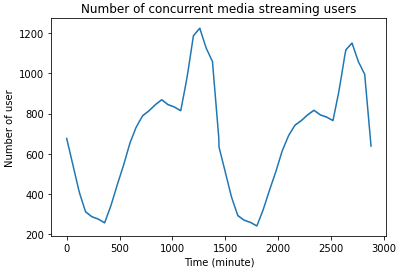
\includegraphics[scale = 0.8]{imgs/media_streaming_concurrent_user_2days.png}
        \caption{Media user generated from user simulation}
        \label{fig:media_user}
    \end{figure}

\begin{figure}[]
    \centering
        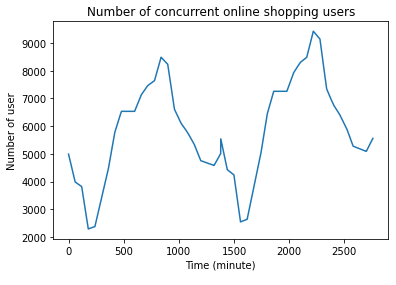
\includegraphics[scale = 0.8]{imgs/online_shopping_concurrent_users_2days.png}
        \caption{Online Shopping user generated from user simulation}
        \label{fig:shopping_user}
    \end{figure}

\begin{figure}[]
    \centering
        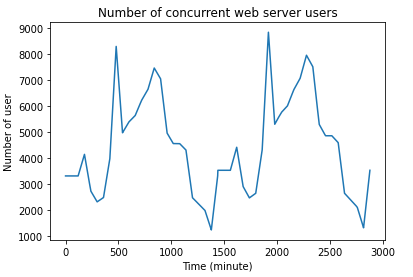
\includegraphics[scale = 0.8]{imgs/web_server_concurrent_user_2days.png}
        \caption{Web server user generated from user simulation}
        \label{fig:webServinguser}
    \end{figure}

\begin{figure}[]
    \centering
        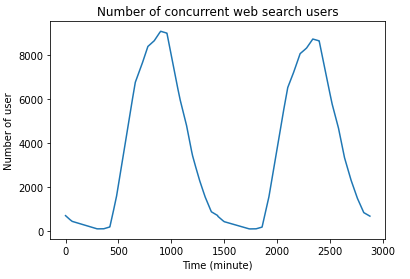
\includegraphics[scale = 0.8]{imgs/web_search_concurrent_users_2days.png}
        \caption{Web searching user generated from user simulation}
        \label{fig:webSearching_user}
    \end{figure}

\subsection{Capturing data}
%TODO: deploy prometheus now/ today ~!!!

NetData has been used to capture the traffic on the link with a sampling rate of 1 second. All the application traffic traces has been captured as in Figure \ref{fig:all_app_resp},\ref{fig:media_resp},\ref{fig:shopping_resp},\ref{fig:search_resp},\ref{fig:serving_resp}. Noted that to speed up, the user generator software scale down the real time to 18 times.

\begin{figure}[]
    \centering
        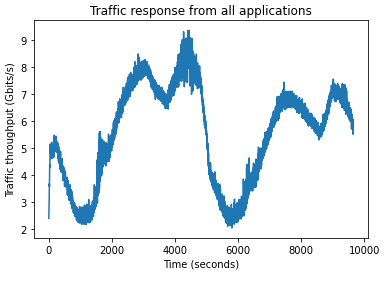
\includegraphics[scale = 0.8]{imgs/agrregated_traffic_all_apps.png}
        \caption{Traffic response from all applications}
        \label{fig:all_app_resp}
    \end{figure}

\begin{figure}[]
    \centering
        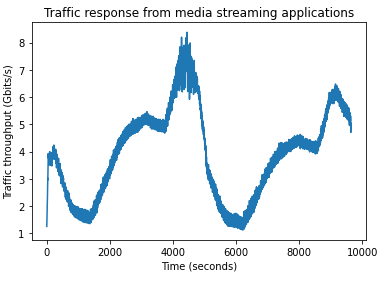
\includegraphics[scale = 0.8]{imgs/media_streaming_response_24_02.png}
        \caption{Traffic response from media streaming application}
        \label{fig:media_resp}
    \end{figure}

\begin{figure}[]
    \centering
        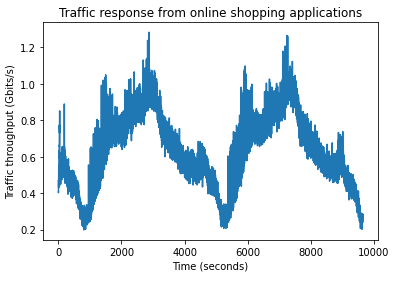
\includegraphics[scale = 0.8]{imgs/online_shopping_response.png}
        \caption{Traffic response from online shopping application}
        \label{fig:shopping_resp}
    \end{figure}

\begin{figure}[]
    \centering
        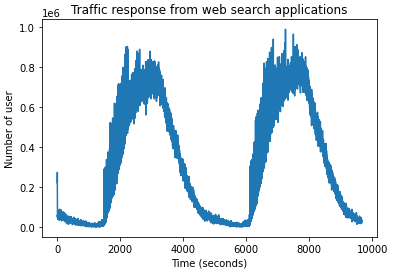
\includegraphics[scale = 0.8]{imgs/search_server_response.png}
        \caption{Traffic response from web search application}
        \label{fig:search_resp}
    \end{figure}

\begin{figure}[]
    \centering
        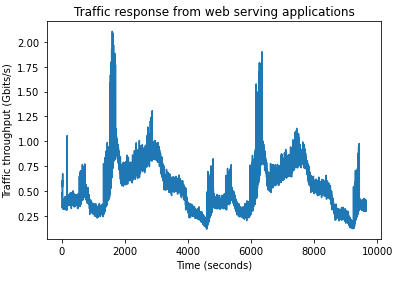
\includegraphics[scale = 0.8]{imgs/web_server_response.png}
        \caption{Traffic response from web server application}
        \label{fig:serving_resp}
    \end{figure}

% section Experiment set up (end)

\section{Simulation}
\label{sec:Simulation}
% section Simulation (begin)

To simulate the optical metro network with edge computing attached to each node and applications as well as client containers in each edge computing, the author proposes a simulation model which combines a network simulator based on OMNET++ and python programming. The optical communication links, buffers, TXs, and WSSs are modeled using the OMNET++ library. Meanwhile, the edge computing server which contains application servers and client containers is modeled using python. 

%TODO: Add a picture to show how the simulation works.

\subsection{OMNET++ software simulator}
OMNeT++ is an extensible, modular, component-based C++ simulation library and framework, primarily for building network simulators. In this work, the OMNET++ software simulation is already built by Bitao. 

Briefly speaking, in this OMNET++ software, during the initial stage, the control packets are sent to establish the time slot in the whole network. The control packets contain a table of the destinations of packets in their time slot. In the running stage, the sources generate the data packets based on pre-defined load parameters to buffer with specify the destination of each packet. The buffer store the data packets from sources in its buffers and then check which wavelength is available and assign the data packet from the most loaded buffer to the available wavelength. In the meantime, the buffer also updates the control packet based on the destination of the data packet. If the buffers are full, the packet from the source would be discarded. The combiner is used to combine the packets from WSS1 and buffer together and put them to the link, which would introduce 100ms latency since the optical link is 20km long. The WSS1 in each node checks the control packet if the data packet coming in that time slot is belongs to the node or not. If the packet does not belong to the node, then the WSS1 just forwards it to the combiner to send it to another node. Otherwise, WSS1 drops the packet to the node and calculate the latency of the packet.

\subsection{Python}

For each specific time, the simulation software calculates the load based on the traffic captured for each application and prepares the initial file for OMNET++ to run. Therefore, each source in a node will represent an application server or a client depends on the deployment action. The action can be to deploy a new application to the network or reallocate an application in the network. In the software, the clients are deployed automatically in every node for each application. For example, with a media application, a media server can be deployed in node 1 and we have clients in all nodes. Therefore there should be 2 sources in node 1, 1 for the media server and the other for the media client and there should be 1 source in every other node for the media client. The load from the server to each client will be split depends on the load request from each client to the server. After the finish preparation stage, the software will use the bash command to run OMNET++ software to do the simulation with specific source loads parameters. After each iteration, the latency, total packet arrival, and packet lost parameter are captured and sent to the control algorithm.

\removelatexerror
\begin{algorithm}[]
    \DontPrintSemicolon
        
        \KwInput{Deployment Action}
        \KwOutput{Network Performance metrics}
        \KwData{Traffic data}

        \For{each data in traffic data}
        {
            \For{each application in deployment action}
            {
                \If{Application is not created yet}
                {
                    Create an application with a particular index.
                }
                \If{Application already belongs to the assigned node or Application application does not belong to any node in the network or Assigned node resources is full}
                {
                    continue - skip the rest of this loop.
                }
                \If{Application currently belongs to another node}
                {
                    Delete the application in that node.
                }

                Deploy the application to the assigned node.

                Deploy users to other nodes.

            }

            Update the source list in each node.

            Create a .ini file from the source list in each node.

            Run OMNET++ software program.

            \If{simulation runtime greater than 10 min}
            {
                Return runtime error.
                
                Stop OMNET++ simulation
            }
            \Else
            {
                Return latency, packet arrival number, packet lost.
            }
        }
    \caption{Simulation Software}
    \label{algo:simulation-python}
\end{algorithm}

\begin{figure}[]
    \centering
        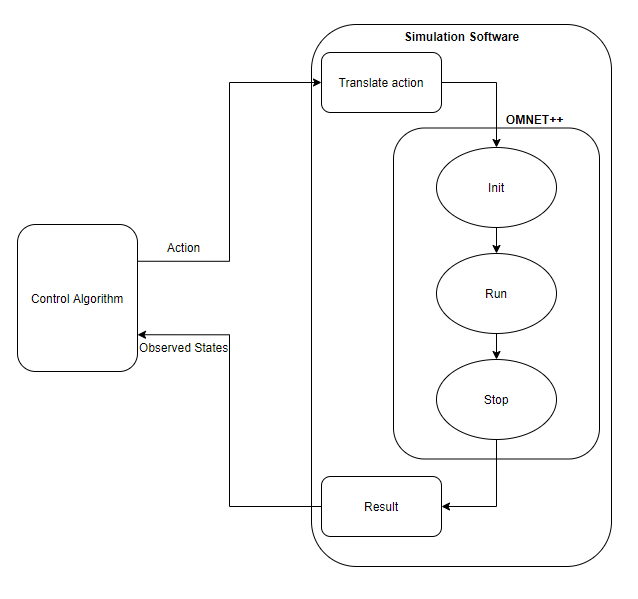
\includegraphics[scale = 0.5]{imgs/Simulation_software.png}
        \caption{Simulation Software}
        \label{fig:simulation_software}
    \end{figure}

% section Simulation (end)

% \section{Algorithm}
% \label{sec:Algorithm}
% % section Algorithm (begin)
% DRL algorithms?
% What is the most potential one?
% What is the one we will use?
% % section Algorithm (end)

\section{Plan}
\label{sec:Plan}
% section Plan (begin)
For the upcoming months, there are several tasks needed to be done.
\begin{itemize}
    \item Investigate the algorithm
    \item Train algorithm with the simulation software
    \item Automate the network with docker swarm or K8s
    \item Train algorithm with real network experiment
\end{itemize}

% section Plan (end)

\bibliographystyle{IEEEtran}
\bibliography{ref/refs.bib}

\end{document}
